\section{Results}

In December of 2013 a total of 10 Bq of tritium was injected into LUX and removed. A total 325,000 events were observed in the active volume of LUX. 140,000 events were collected in the fiducial volume at the nominal LUX electric field of 180 V/cm, while 4,500 fiducial events were collected in a special run at a reduced field of 100 V/cm. The S1 and S2 signals are corrected for spatial effects such as the light collection efficiency and the free electron lifetime with $^83m$Kr data as described in \cite{lux-reanalysis}. 

We interpret the data in terms of the combined energy model \cite{platzman}, where the total energy of an event is directly proportional to the number of quanta produced (electrons pus scintillation photons):

\begin{displaymath}
\rm E_{total} = W \cdot (n_{\gamma} + n_e )
\end{displaymath}

\noindent
We use a $W$ value of 13.7 eV/quanta \cite{Dahl_Thesis}. In LUX $n_{\gamma}$ and $n_e$ are proportional to the S1 and S2 signals, with gain factors $g_1$ and $g_2$:

\begin{displaymath}
\rm E_{total} = W \cdot \left(\frac{S1}{g_1} + \frac{S2}{g_2} \right)
\end{displaymath}

\noindent
where S1 and S2 have units of \fixit{phe} and $g_1$ and $g_2$ have units of phe per quanta. $g_1$ is the average light collection efficiency times the average quantum efficiency of the PMT arrays, while $g_2$ is the product of the electron extraction efficiency at the liquid-gas surface, the secondary scintillation gain factor, and the average PTM quantum efficiency. $g_1$ and $g_2$ are measured with line source data in LUX as described in Ref. \cite{lux-reanalysis, lux-prd}. We find values of \fixit{$g_1$ = \gone and $g_2$ = \gtwo}.

\begin{figure}[h!]\centering
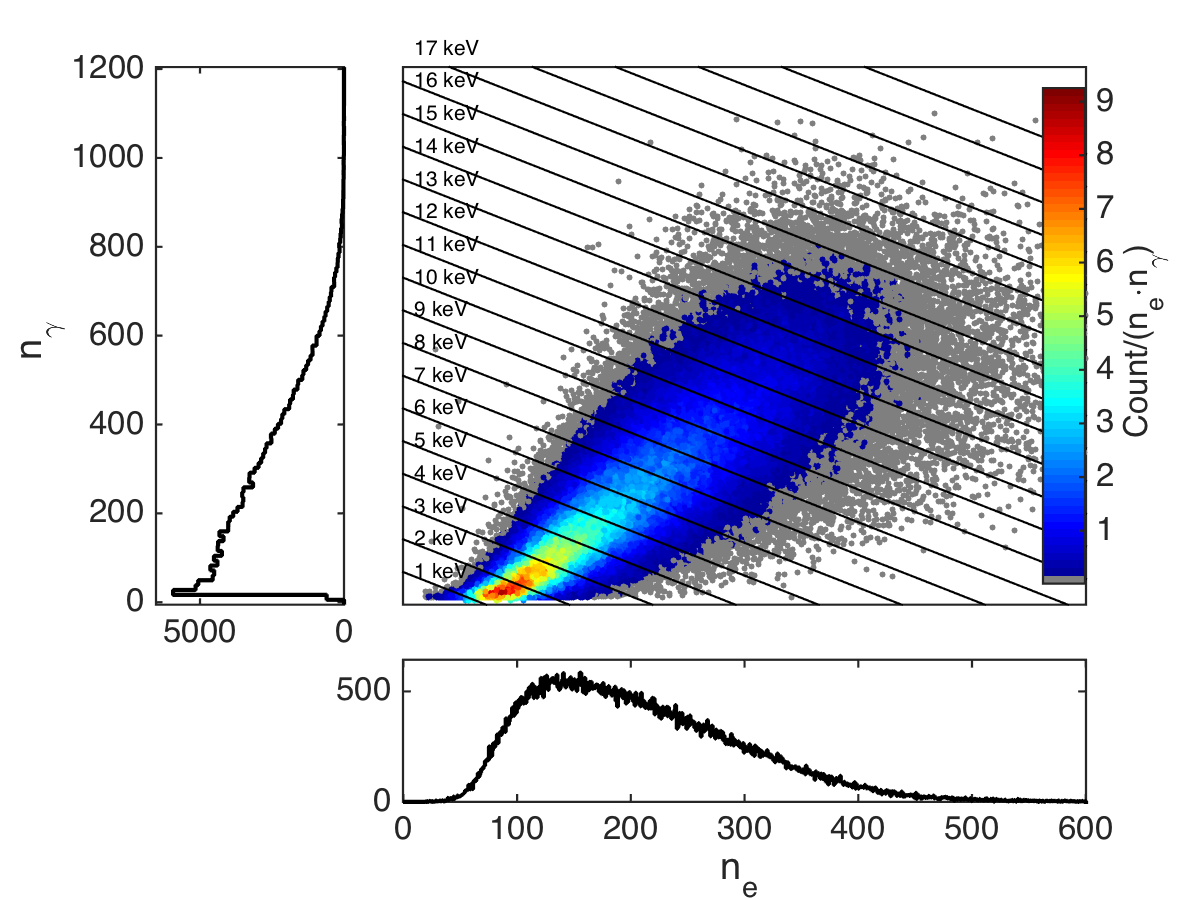
\includegraphics[width=90mm]{fig/tritium_scatter.png}
\caption{Scatter plot of $n_e$ vs $n_{\gamma}$ for 115,000 fiducial tritium events at 180 V/cm. Lines of constant energy are indicated assuming a $W$ value of 13.7 eV/quanta. The data is projected into $n_e$ and $n_{\gamma}$ histograms on each axis.}
\label{fig:tritium_scatter}
\end{figure}


\begin{figure}[h!]
\begin{center}
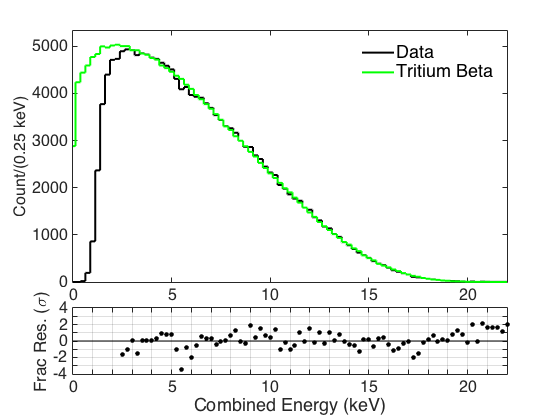
\includegraphics[width=90mm]{fig/tritium-spectrum-linear.png}
\caption{The tritium energy spectrum measured by LUX with the combined energy model (black) compared to several theory models: a pure tritium spectrum (dashed blue), LUXsim (red) and a tritium spectrum with a simple energy smearing of $\sigma_E = XXXX$ applied. }
\label{fig:tritium-spectrum}
\end{center}
\end{figure}



A scatter plot of $n_e$ vs $n_{\gamma}$ for the tritium data at 180 V/cm is shown in Fig. \ref{fig:tritium-scatter}, along with the projected histograms on each axis. The tritium energy spectrum, obtained by projecting the data along the lines of constant energy, is shown in Fig. \ref{fig:tritium-spectrum}. The data is compared to several models: a pure tritium spectrum, with no detector effects; a spectrum simulated with LUXsim, and a tritium spectrum with a simple energy smearing factor of $\sigma_E = XXXX$ applied. The ratio of the data to the smeared tritium spectrum is shown in Fig. \ref{fig:ER-threshold}, along with a fit to an error function. The ratio indicates that the data is well modeled by the smeared tritium spectrum, and the effective 50\% energy threshold is found to be 1.04 $\pm$ 0.016 keV. 

\begin{figure}[h!]\centering
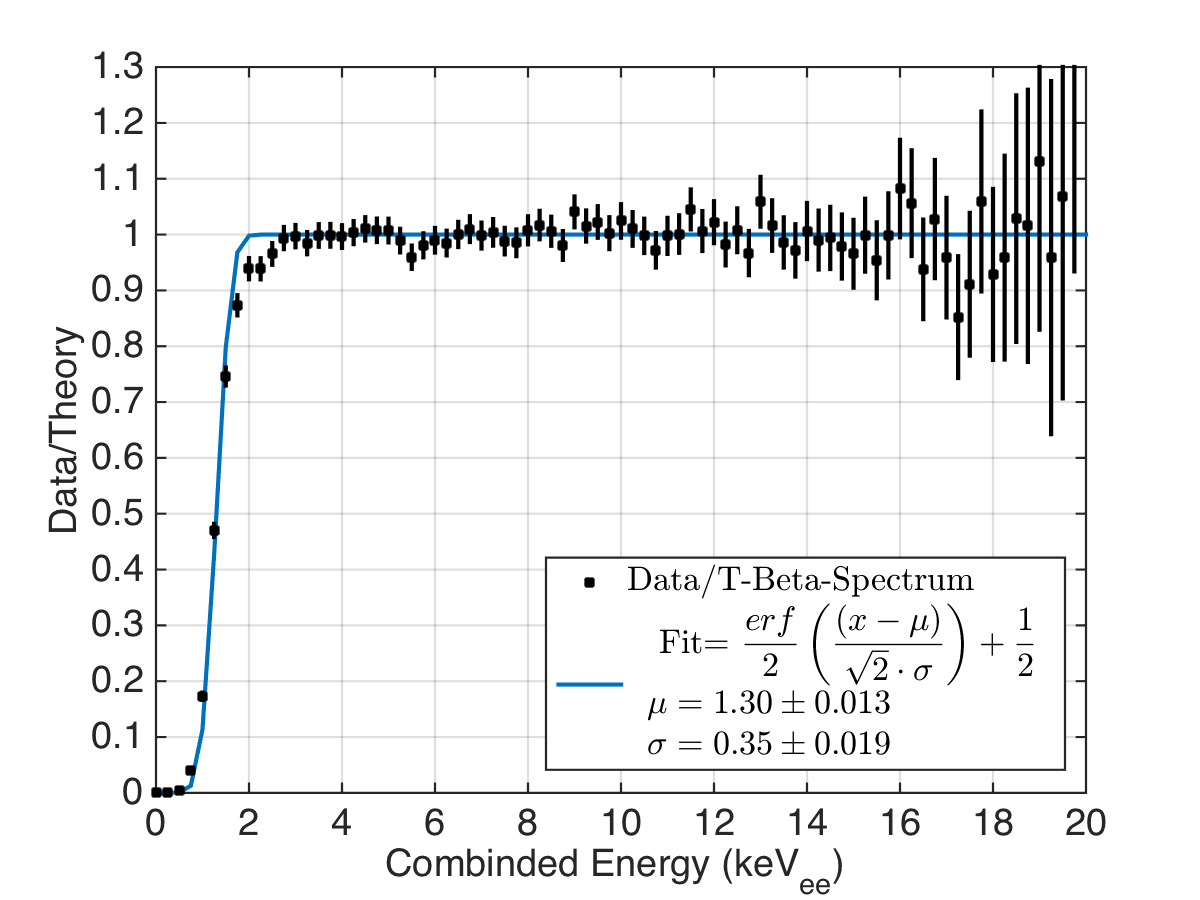
\includegraphics[width=90mm]{fig/E_Thres_Fit.png}
\caption{ER threshold measured by comparing the measured energy spectrum to the smeared tritium spectrum. A fit to an error function is shown.}
\label{fig:ER-threshold}
\end{figure}

The mean light yield and charge yield of ER events in LUX are obtained by dividing the mean light and charge signals by the combined energy in each energy bin. The result is shown for 180 V/cm in Fig. \ref{fig:ER-LY-QY}. For these plots a small correction has been applied to the data to account for smearing of tritium events across energy bins due to the detector's resolution \cite{Dobi_Thesis}. 

\begin{figure}[h!]\centering
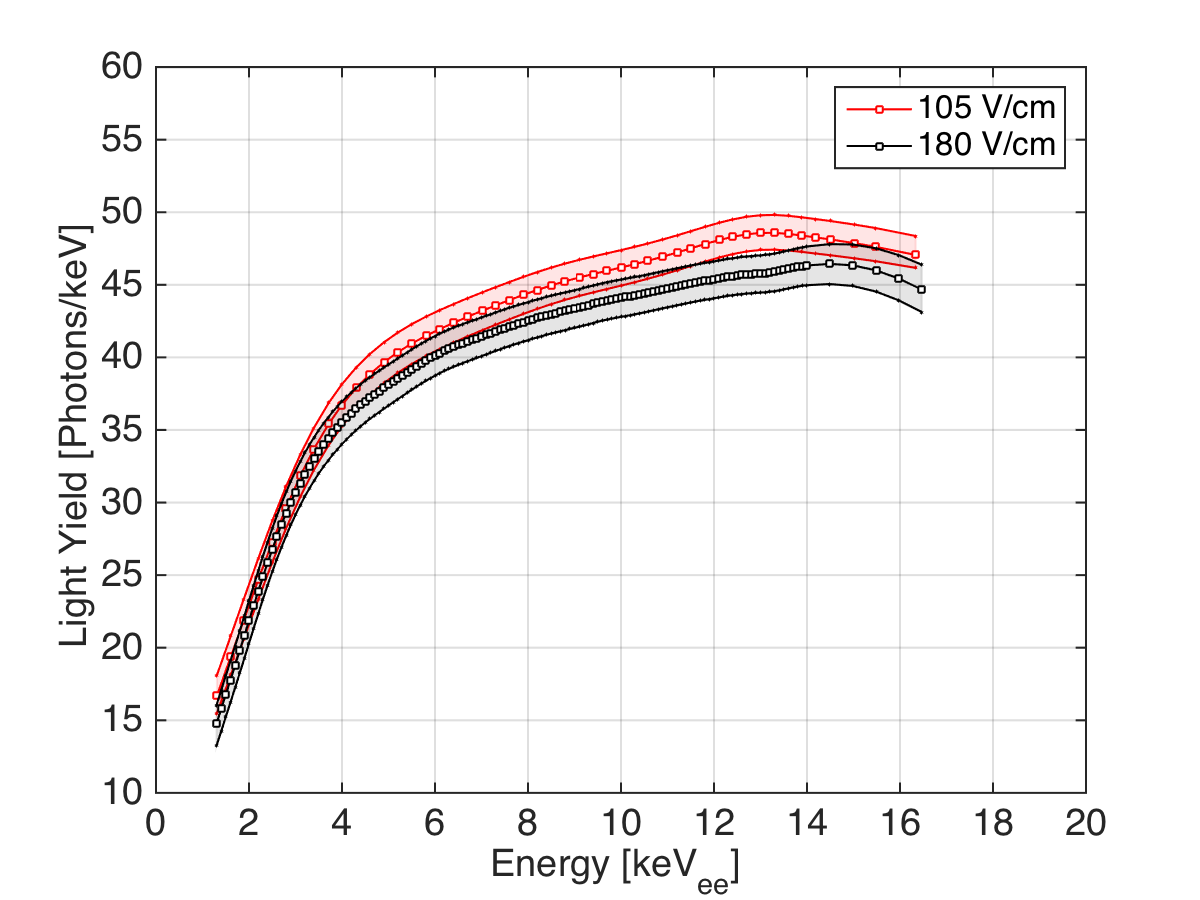
\includegraphics[width=90mm]{fig/ER_LY.png}
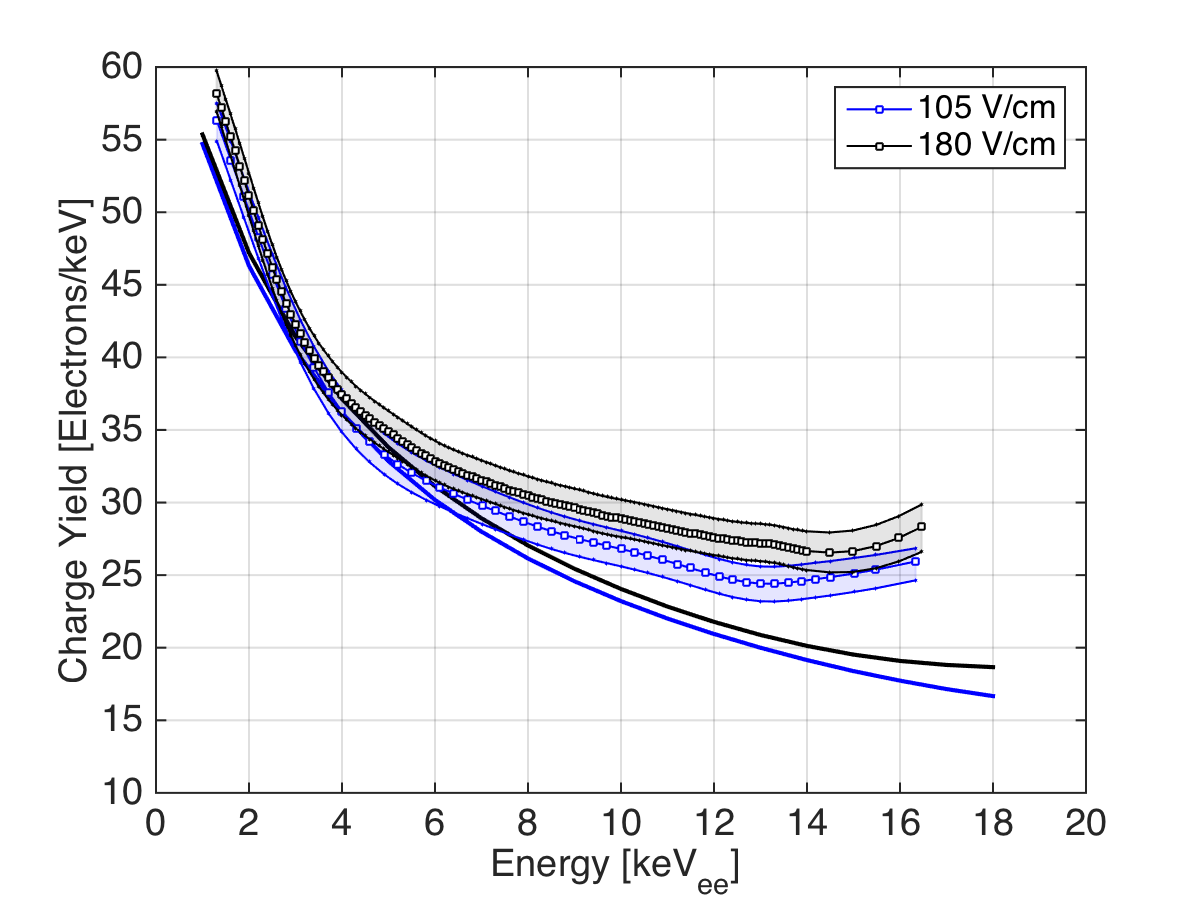
\includegraphics[width=90mm]{fig/ER_QY.png}
\caption{The light yield and charge yield of ER events in LUX at 180 V/cm compared to NEST v0.98 (2013). The grey bands indicate the systematic errors on $g_1$ and $g_2$, which are fully correlated across all energy bins. $g_1$ is anti-correlated with $g_2$, such that an increase in the charge yield within the grey band must be compensated by an equivalent decrease in the light yield. Upper: Light yield at 180 V/cm. Lower: the charge yield at 180 V/cm.}
\label{fig:ER-LY-QY}
\end{figure}

 \begin{figure}[h!]\centering
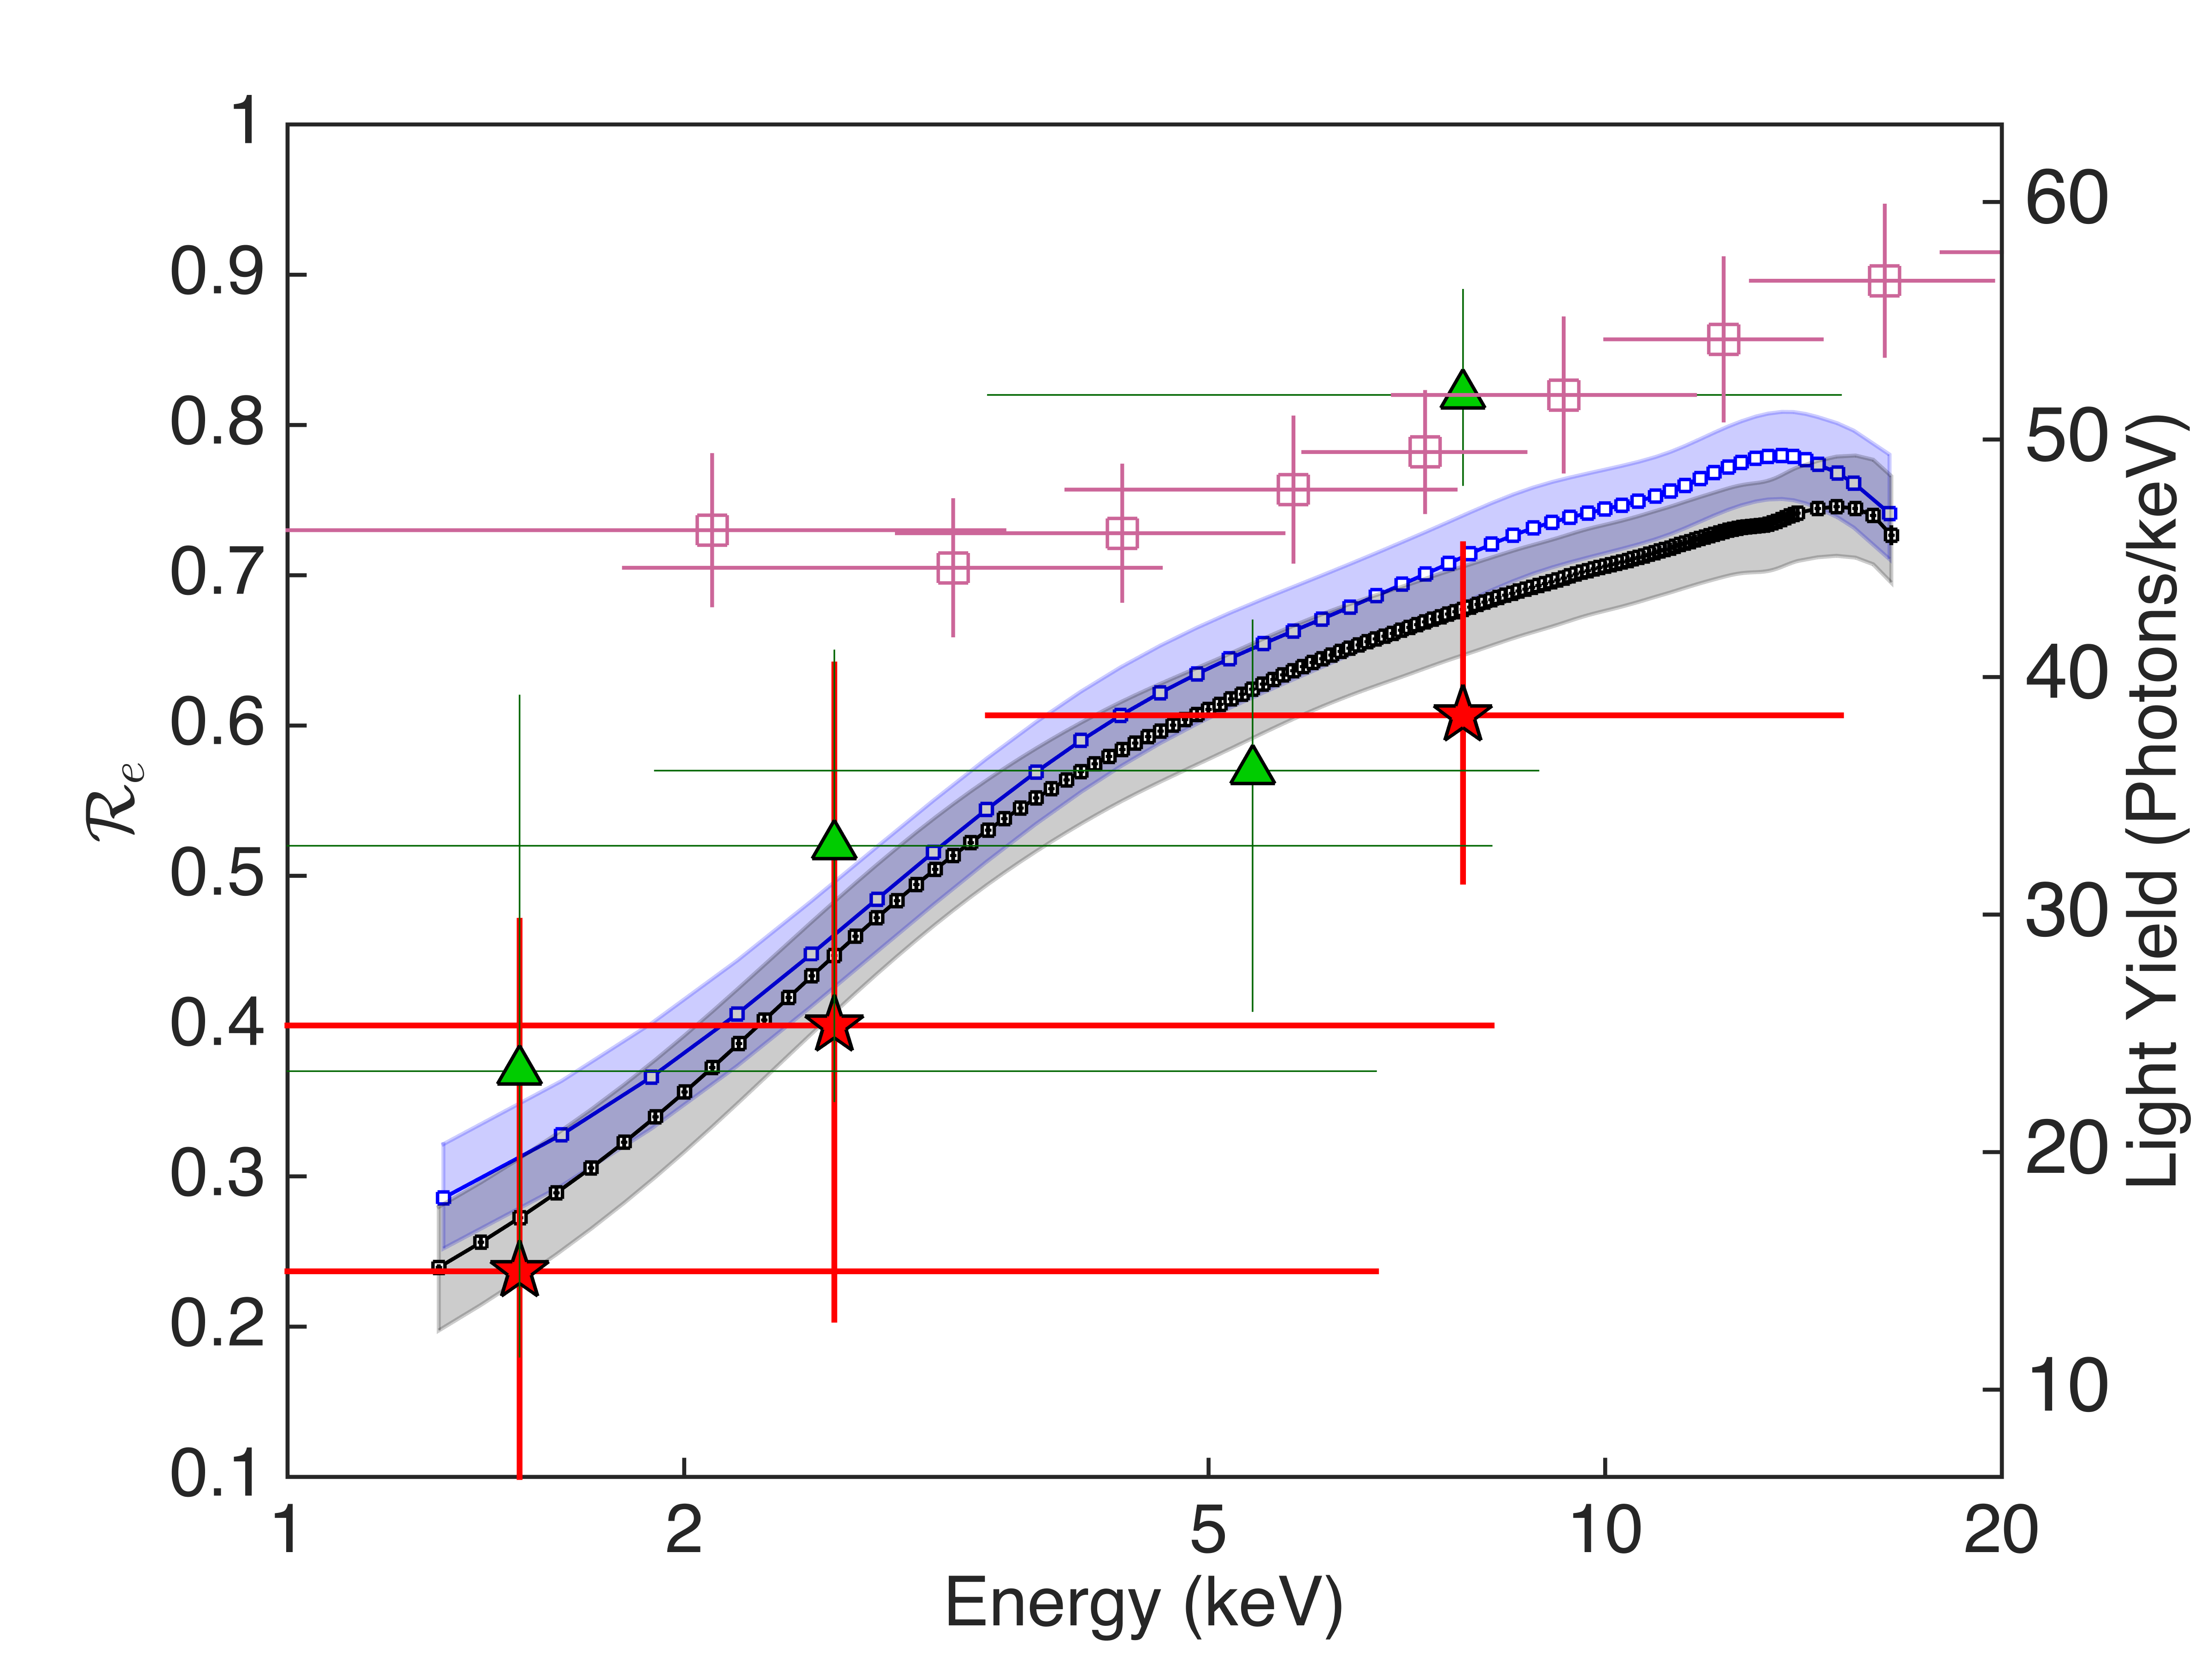
\includegraphics[width=88mm]{fig/Re_LY_log.png}
\caption{Scintillation yield relative to the yield of the 32.1 keV decay $\rm^{83}Kr $  vs. Energy. Shaded blue curve is tritium at 100 [V/cm], shaded black curve is tritium at 180 [V/cm], red circles represent a recent Compton scattering measurement at 450 [V/cm]. }
\label{fig:Re_LY}
\end{figure}


\begin{figure}[h!]\centering
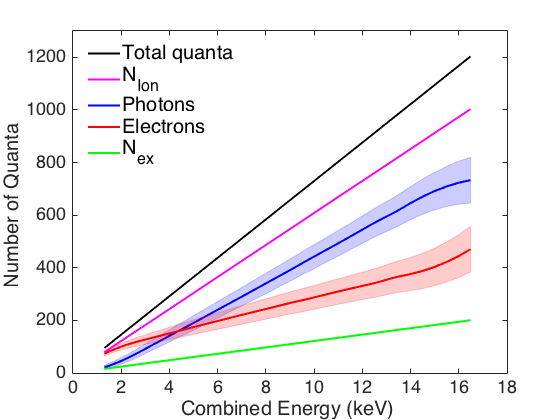
\includegraphics[width=90mm]{fig/quanta-vs-energy.png}
\caption{The mean number of electrons (red) and scintillation photons (blue) produced in LUX at 180 V/cm as a function of energy. The bands indicate the correlated systematic errors on $g_1$ and $g_2$. Also shown are the total number of quanta, primary ions, and primary excitons, assuming an exciton to ion ratio of 0.2. }
\label{fig:quanta-vs-energy}
\end{figure}


\begin{figure}[h!]\centering
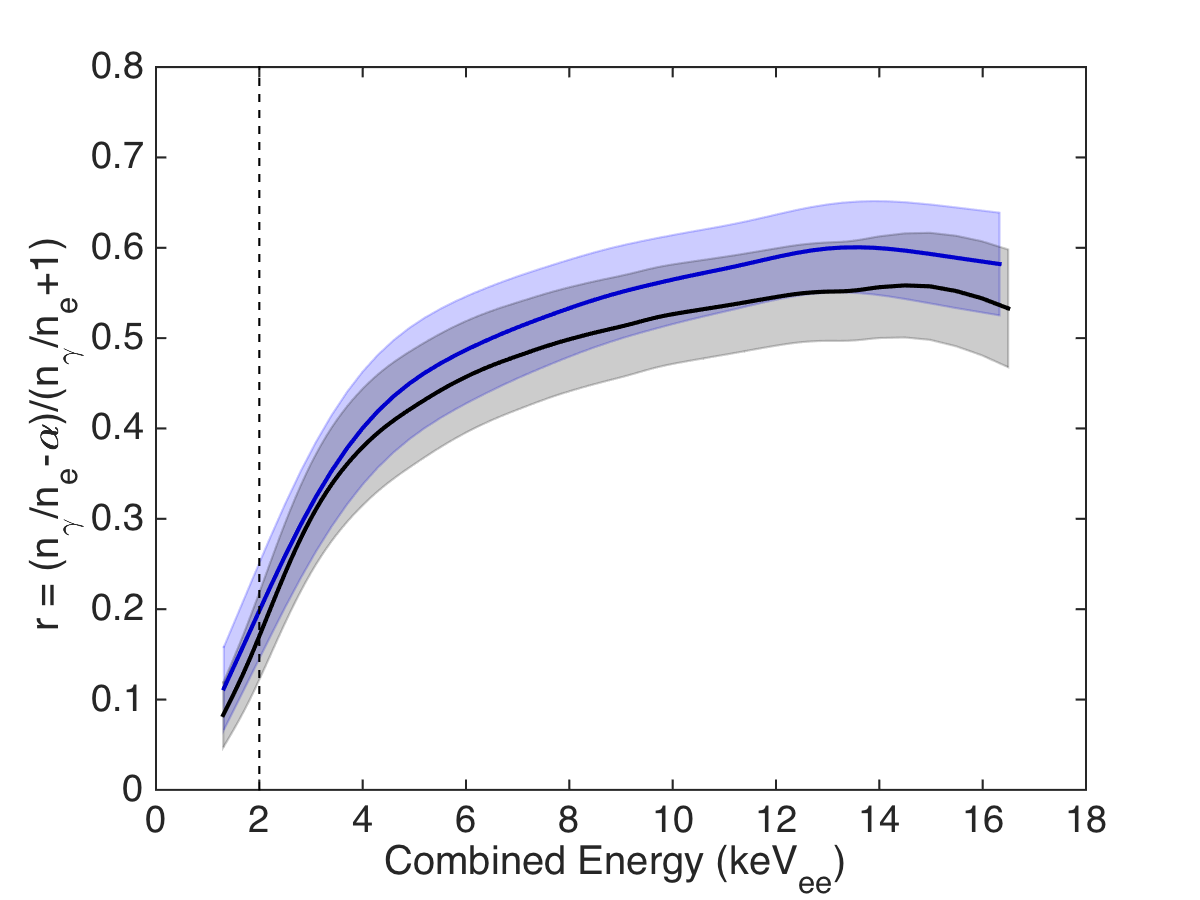
\includegraphics[width=90mm]{fig/recombination.png}
\caption{Recombination fraction of ER events at 180 V/cm, assuming an exciton-to-ion ratio of 0.2.}
\label{fig:recombination}
\end{figure}


As shown in Fig. \ref{fig:ER-LY-QY}, the light yield is observed to drop rapidly between 1 and 6 keV, and then becomes mostly energy independent over the remainder of the tritium spectrum. The charge yield exhibits the reverse behavior. These effects can also be illustrated by plotting the total number of quanta as a function of energy, as shown in Fig. \ref{fig:quanta-vs-energy} for tritium events between 1 and 8 keV. Also shown in Fig. \ref{fig:quanta-vs-energy} are the total number of quanta assuming a $W$ value of 13.7 eV/quanta (black), and the primary number of ions (violet) and excitons (cyan) prior to recombination assuming an initial exciton-to-ion ratio of 0.2 \cite{alpha-value}. We interpret the charge yield data as a measure the recombination fraction at each energy according to

\begin{displaymath}
r = \frac{\frac{n_{\gamma}}{n_e} - \alpha}{\frac{n_{\gamma}}{n_e} + 1}
\end{displaymath}

\noindent
where $r$ is the recombination fraction and $\alpha$ is the initial exciton-to-ion ratio. The recombination fraction as a function of energy as shown in Fig. \ref{fig:recombination}. Here the falling charge yield and rising light yield between 1 and 6 keV appears as a rapid rise in the recombination fraction. 

\begin{figure}[h!]\centering
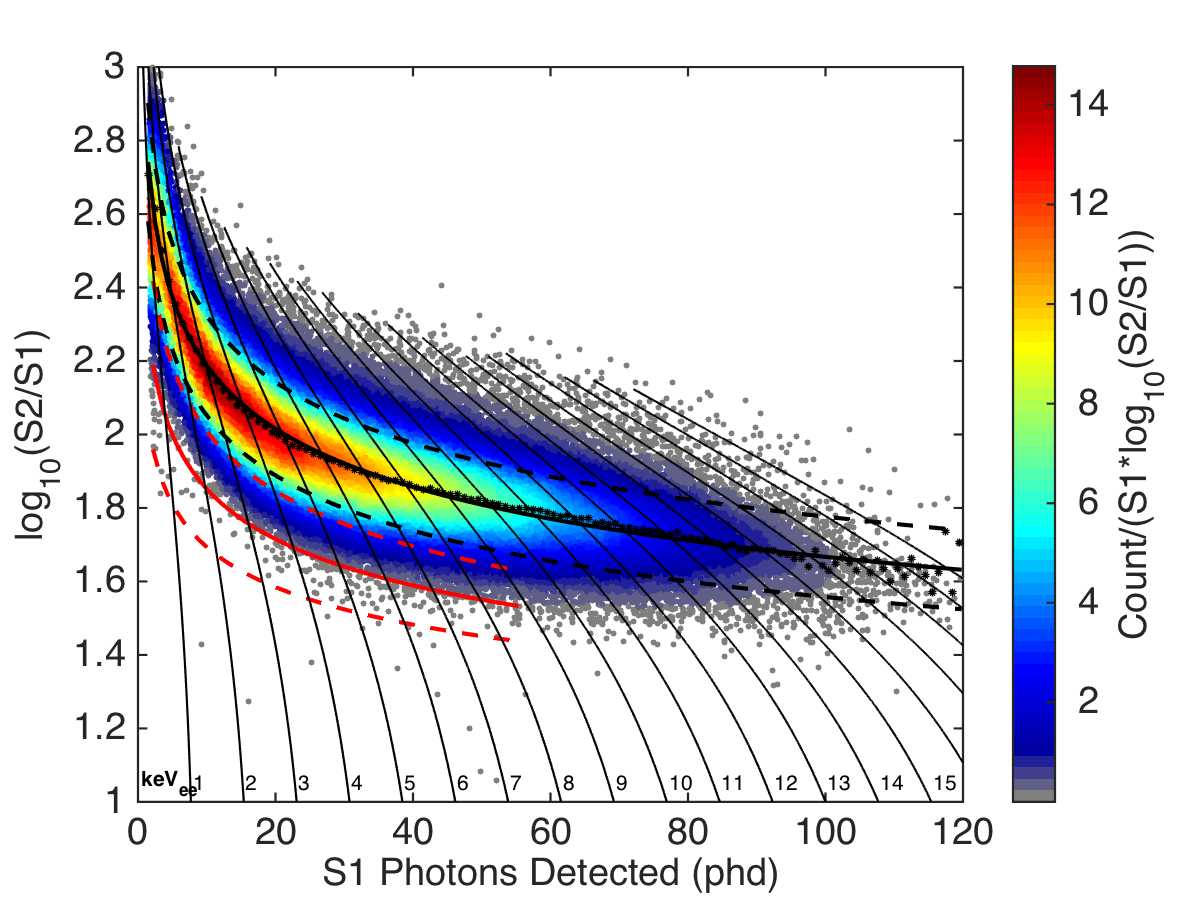
\includegraphics[width=100mm]{fig/CH3T_ER_Band.png}
\caption{The electron recoil band of LUX illuminated by 115,000 tritium events at the nominal LUX electric field of 180 V/cm.  The recoil discriminant variable, log(S2/S1), is shown vs. S1 between 1 and 50 phe in S1 (about $\rm1-8 keV_{ee}$). Also indicated in black are the mean and the 10\% and 90\% contours. The solid red line represents the mean NR band determined with NEST v0.98 (2013) \cite{nest} and validated with AmBe and $\rm^{252}Cf$ neutron sources and the DD neutron generator data. The dashed red indicates the 10\% and 90\% contours of the NR band.}
\label{fig:ER_band}
\end{figure}

We obtain the LUX ER band by plotting log$_{10}$(S2/S1) vs S1 as shown in Fig. \ref{fig:ER_band}. Also shown is the LUX NR band determined with NEST v0.98 (2013) \cite{nest} and validated with AmBe and $\rm^{252}Cf$ neutron sources and DD neutron generator data. The ER band has a characteristic rise at low S1 which reflects the increasing charge yield and decreasing light yield below 4 keVee, as seen in Fig. \ref{fig:quanta-vs-energy}. The leakage fraction ($f$), defined as the fraction of ER events that fall below the mean of the NR band, is shown in Fig. \ref{fig:Leak} as a function of S1. The recoil discrimination ($1-f$) has an average value of \fixit{99.58\%} for events with S1 between 1 and 30 phe.


\begin{figure}[h!]\centering
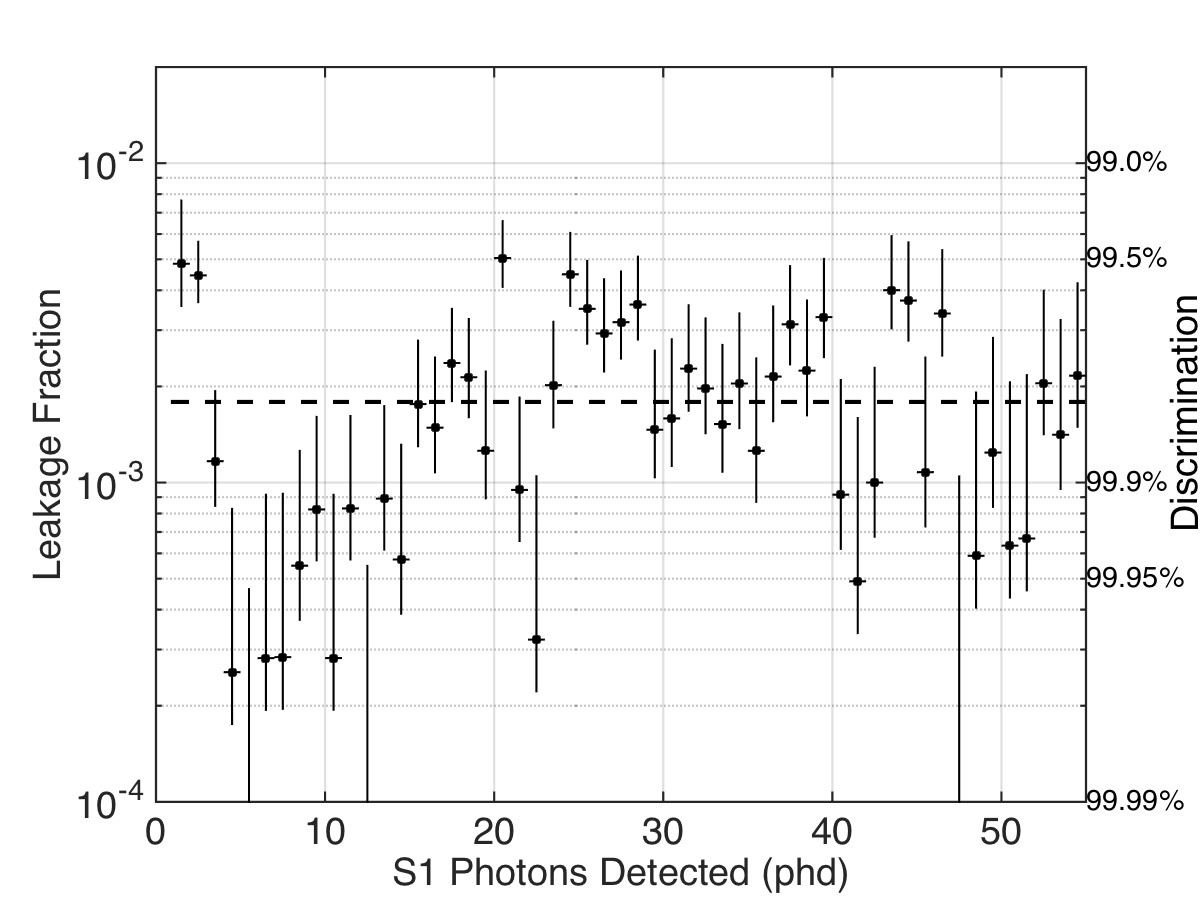
\includegraphics[width=90mm]{fig/CH3T_Leakage_Run03.png}
\caption{LUX recoil discrimination vs. S1, determined from Fig. \ref{fig:ER_band}. Y-axis labels: left -  leakage fraction ($f$); right - discrimination ($1-f$).}
\label{fig:Leak}
\end{figure}

%%%%%%%%%%%%%%%%%%%%%%%%%%%%%%%%%%%%%%%%%%%%%%%%%%%%%%%%%%

